\documentclass{beamer}
\usepackage[utf8]{inputenc}
\usepackage{verbatim}
\usepackage{graphicx}
\usepackage{multicol}
\usetheme{Berlin}
\usecolortheme{beaver}
\usepackage{color}
\newcommand{\norm}[1]{\left\lVert#1\right\rVert}
\graphicspath{ {images/} }

\begin{document}
\title{The Lasso Method of Parameter Selection}
\author{C. Kinstley, A. Nabar, T. Williams, C. Vollmer }
\frame{\titlepage}

\section[Outline]{}
\frame{
\begin{multicols}{2}
 \tableofcontents[%pausesections
 ]
 
 \end{multicols}
}

\section{Improving OLS}

\frame{
\begin{multicols}{2}
 \tableofcontents[currentsection, hideothersubsections]
\end{multicols}
}

\frame
{
\frametitle{Improving OLS}
	\begin{itemize}
	\item Recall the ordinary least squares procedure (OLS) estimates unknown coefficients in a linear regression model by minimizing the {\color{red}squared difference} between the {\color{purple}predicted} and {\color{blue}actual} responses. 
	
	\item We would like to fit $n$ data points to a model of the form {\color{purple}$$y= \beta_0 + \beta_1 x_1 + \beta_2 x_2+ \dots +\beta_{p-1} x_{p-1}+\color{red}\epsilon$$}
	
	\item Let $X$ denote the $n \times p$ design matrix where the $x_{ij}$th entry is the $i$th point of sample data corresponding to the $j$th dependent variable and $Y$ the response vector
		

	\end{itemize}
}



\frame
{
\begin{itemize}

	\item  So long as $n \geq p$, OLS gives us a best-fit hyper-plane as follows:
    
    \begin{itemize}
    \item The {\color{red}difference}, or the error, between the actual and 
    predicted response for each data point $i \in 1 \dots n$ is
    
    \begin{equation*}
     {\color{red} \epsilon_{i}} =  {\color{blue} Y_{i}} - {\color{purple} X\beta}
     \end{equation*}
    
    \item We minimize the sum of the squared differences, i.e minimize the function
    $$ E({\color{purple}\hat{\beta} }) = \sum_{i=1}^n {\color{red}{\epsilon_i^2}} = \norm{{\color{blue}Y}^2_2- {\color{purple}X\beta}}_2^2$$
    
    \item It can be shown that the minimizers are
    $\hat{\beta} = (X^TX)^{-1}X^TY$ but these solutions are usually approximated.
    \end{itemize}
    
\end{itemize}
}

\subsection{What can be improved?}
\frame
{

  \frametitle{Problems with OLS}
  
  Two common problems with OLS estimates are as follows:
  \begin{itemize}
  \item Imprecision
  \item The expected value of the error term is 0 but the variance may be large.
  \item How does this happen? Recall that the least squares estimation $\hat{\beta} = (X^T X)^{-1}X^T Y$.
        \item If $(X^T X)$ is near-singular, then small changes in the X might lead to large changes in $\hat{\beta}$.
        \item So, even if our $\hat{\beta}$ fits one sample well, there is no guarantee it will fit other samples well, let alone the population! 
\end{itemize}
}
        
        
\frame{
        
\begin{itemize}        
\item Interpretation
\item A large number of independent variables can make the model difficult to interpret, especially when we want to isolate the "most important" variables.
\item Do we care about variables with very small coefficients?
\end{itemize}
}


\subsection{Subset Selection \& Ridge Regression}
\frame{
\frametitle{Improving OLS: Subset Selection}
Subset Selection
    \begin{itemize}
\item Simply ignore one or more of the independent variables! That is, set the coefficient(s) to 0.
\item This helps with interpretability, if only because there is less to interpret.
\item Drawback: Subset Selection is a discrete process. Regressors are either kept or dropped; there is no in-between. Small changes in the sampling data can thus result in very different models.
\item Not computationally practical for high dimensional data.
\end{itemize}
}

\frame{
\frametitle{Improving OLS: Ridge Regression}
Ridge Regression
\begin{itemize}
\item In Ridge regression we again minimize $E(\beta) = \norm{Y-X\beta}_2^2$
\item But subject to the constraint that $$\sum_{i=1}^{p-1}\beta_i^2 = \norm{\beta}_2^2 \leq t \ \text{for} \ t\geq 0$$
\end{itemize}

}


\frame{
\frametitle{Improving OLS: Ridge Regression}
Ridge Regression
\begin{itemize}
\item This is equivalent to the unconstrained minimization of
\[
E^R(\beta)=\norm{Y=X\beta}_2^2 + \lambda \norm{\beta}_2^2
\]
where $\lambda$ is a function of $t$
\end{itemize}

}


\frame{
\frametitle{Improving OLS: Ridge Regression}
Ridge Regression
\begin{itemize}
\item In terms of the coefficients, $\hat{\beta}^{R}$, it is equivalent to adding a small constant value $\lambda$ to diagonal entries of $(X^T X)$ in the OLS solution
\item This prevents the matrix from being singular or near-singular.
\item Drawback: Reduces the variance of the error term, but does not set any coefficients to 0, so it doesn't help with interpretability. It also adds bias.
\end{itemize}

}

\section{Lasso}

\frame{
\begin{multicols}{2}
 \tableofcontents[currentsection, hideothersubsections]
\end{multicols}
}


\frame{
    \frametitle{Enter the Lasso}
    \begin{itemize}
        \item L.A.S.S.O: Least Absolute Shrinkage and Selection Operator.
        \item Like Ridge we minimize $E(\beta)$ under a constraint, the lasso coefficients are found by minimizing
        \[
        E^L(\beta) = \norm{Y-X\beta}_2^2 \text{ subject to } \norm{\hat{\beta}}_1^2 \leq t
        \]
        \item We are using the 1 norm, instead of the 2 norm used in ridge
        \item As in Ridge this can be written as an unconstrained optimization problem with $\lambda (t)$
    \end{itemize}

}


\subsection{Variable Selection}
\frame{
\frametitle{Variable Selection}
\begin{itemize}
\item Lasso has the desirable property that it will usually set some of the coefficients equal to zero 
\item Like in subset selection this leads to a more interpretable model overall
\item In Ridge and OLS the minimizing coefficients are almost certainly non-zero
\end{itemize}
}

\frame{
\frametitle{Why is this?}
Consider the constrained optimization problems for lasso and ridge in the case of two variables

\center{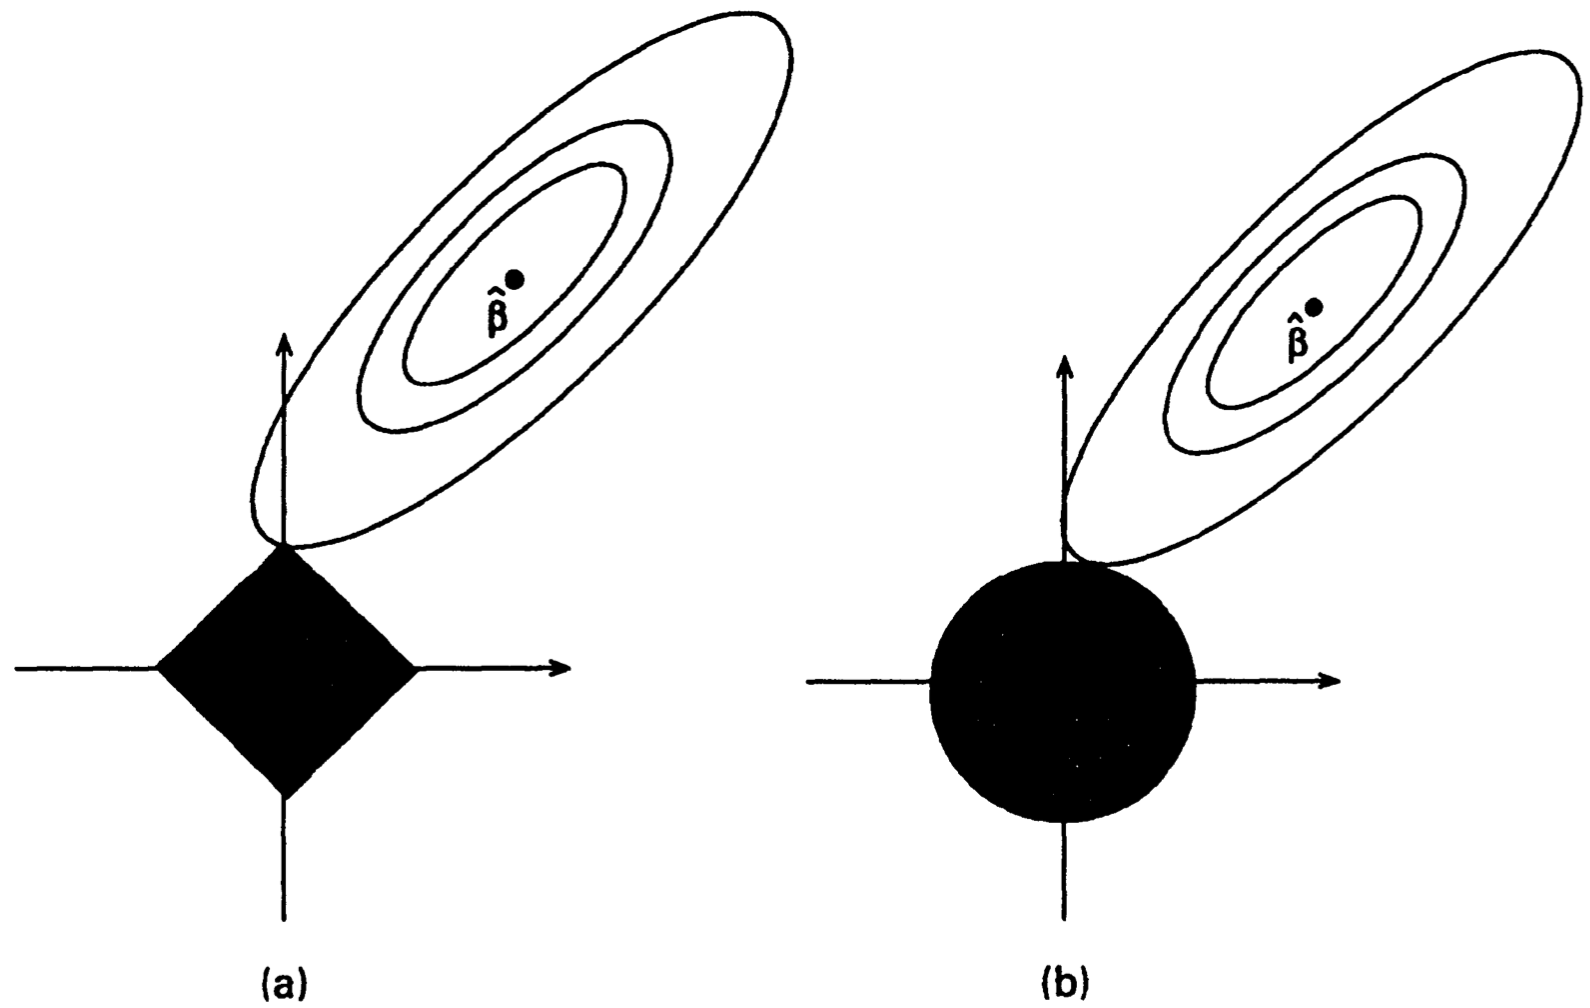
\includegraphics[scale=.25]{tibfig2}}

}


\addtocontents{toc}{\newpage}
\section[Tuning Parameter]{Tuning Parameter}

\subsection[Tuning Parameter]{}
\frame{
\begin{multicols}{2}
 \tableofcontents[currentsection, hideothersubsections]
\end{multicols}
}


\frame{
    \frametitle{Tuning parameter}
    In order to obtain an optimal estimate, of the $\hat{\beta}$ coefficients, the tuning parameter $t$ must be chosen carefully. Recall that in ridge regression,
    \[
    E_R(\beta) = \norm{Y - X\beta}_1^2 + \lambda \norm{\beta}_2^2 = OLS + \lambda \norm{\beta}_2^2
    \]
    the least squares component is being minimized with the constraint 
    \[
    \lambda \norm{\beta}_2^2 = \sum_{j=1}^p {\beta_j^2} \le t
    \]
    }
     
    
\frame{
    \frametitle{Tuning parameter}
    Similarly, remember that the Lasso method 
    \[
    E_R(\beta)= \norm{Y-X\beta}_1^2 + \lambda \norm{\beta}_1^2 = OLS + \lambda \norm{\beta}_1^2
    \]
    is minimizing the least squares component given the constraint  
    \[
    \lambda \norm{\beta}_1^2 = \sum_{j=1}^p {|\beta_j|} \le t
    \]
} 

\frame{
        \frametitle{Tuning parameter}
        Tuning parameter $t$ or $\lambda(t)$ directly determines the amount of shrinkage applied to the OLS estimates.
        \begin{itemize}
        \item Consider the OLS estimates as vector $\hat{\beta}^{ols}$. 
        % \linebreak $\hat{\beta}^{ols} = 
        % \begin{bmatrix}
        %   \hat{\beta}_{1} \\
        %   \hat{\beta}_{2} \\
        %   \vdots \\
        %   \hat{\beta}_{p}
        %  \end{bmatrix}$ 
         \item Define $t_{ols} = \sum_{j} |\hat{\beta}_{j}|$. 
         \item When $t \geq t_{ols}$, we recover the OLS estimates. It follows then that setting $t \leq t_{ols}$ will \color{red} shrink \color{black} the solutions toward 0. 
         \item Setting $t \leq t_{0}$ will \color{red} shrink \color{black} the solutions toward 0.
         \item For example, setting $t = \frac{t_{0}}{2}$ is similar to selecting the best subset containing half of the regressors.
    \end{itemize}
}

% \frame{
% \frametitle{Tuning parameter}
%      \begin{itemize}
%          \item Setting $t \leq t_{0}$ will \color{red} shrink \color{black} the solutions toward 0.
%          \item For example, setting $t = \frac{t_{0}}{2}$ is similar to selecting the best subset containing half of the regressors. 
%     \end{itemize}
            
% }



\frame{
\frametitle{Why is this?}
In the 2-D case, the constraint $t$ can be depicted as follows.
\center{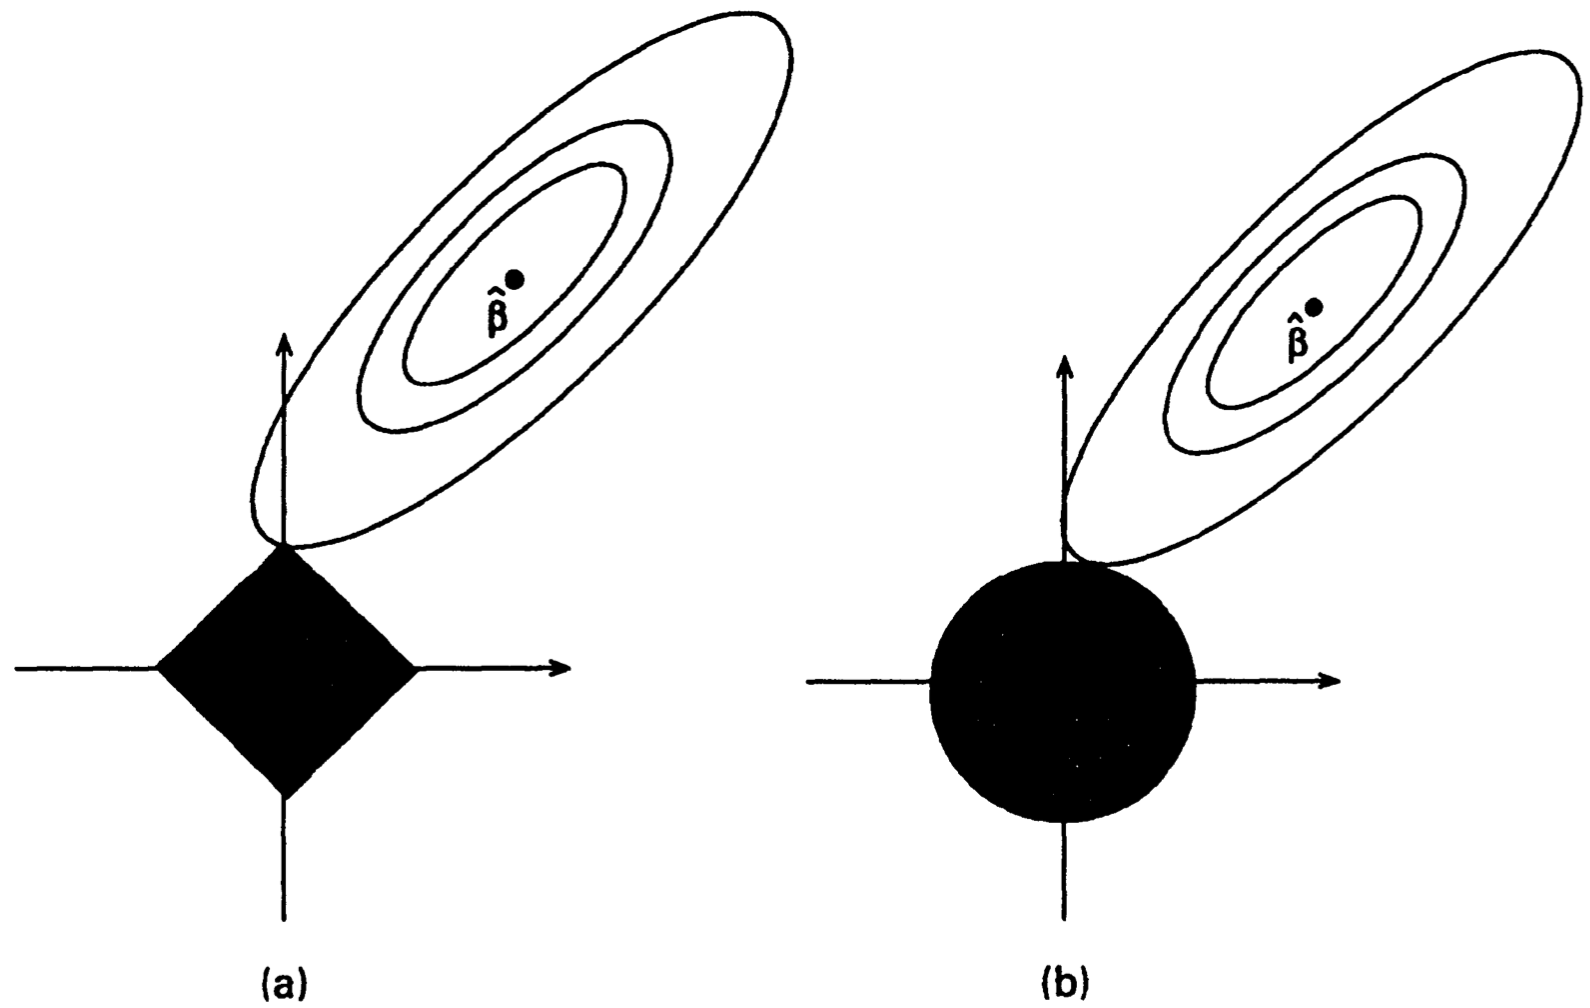
\includegraphics[scale=.25]{tibfig2} 
}}


\frame{
\frametitle{Selecting t or $\lambda(t)$}
    \begin{itemize}
        \item
        In the equivalent unconstrained problem $\lambda(t)$ is a function of t
        \[
        E^L(\beta)=\norm{Y-X\beta}_2^2 + \lambda \norm{\beta}_1^2
        \]
    \end{itemize}
}

\frame{
    \frametitle{Methods for selecting $t$}
    There are a number of methods used to estimate lasso parameter $t$. We will be covering
    \begin{itemize}
        \item Cross-validation
        \item Bayesian information criteria (BIC)
        \item Shooting method
    \end{itemize}
}

\subsection{Cross-Validation}

\frame{
    \frametitle{Cross-validation}
}

\subsection{BIC}

\subsection{Shooting Method}


%Examples
\section{Examples}

\frame{
\begin{multicols}{2}
 \tableofcontents[currentsection, hideothersubsections]
\end{multicols}
}



\subsection{Prostate Cancer}

\frame{
    \begin{itemize}
        \item This prostrate cancer data comes from a study by Stamey et al. (1989) that examined the correlation between the level of prostrate specific antigen and a number of clinical measures.
        \item Our regressors are log(cancer volume) (lcavol), log(prostrate weight) (lweight), age, log(benign prostatic hyperlasia amount) (lbph), seminal vesicle invasion (svi), log(capsular penetration) (lcp), Gleason score (gleason) and percentage Gleason scores 4 or 5 (pgg45).
        \item This graph exhibits the lasso shrinkage of the coefficients; each curve represents a lasso coefficient as a function of the scaled lasso parameter s = t/sum; the broken line represents the model for s hat = 0.44, selected by generalized cross-validation
    \end{itemize}
}

\frame{

\center{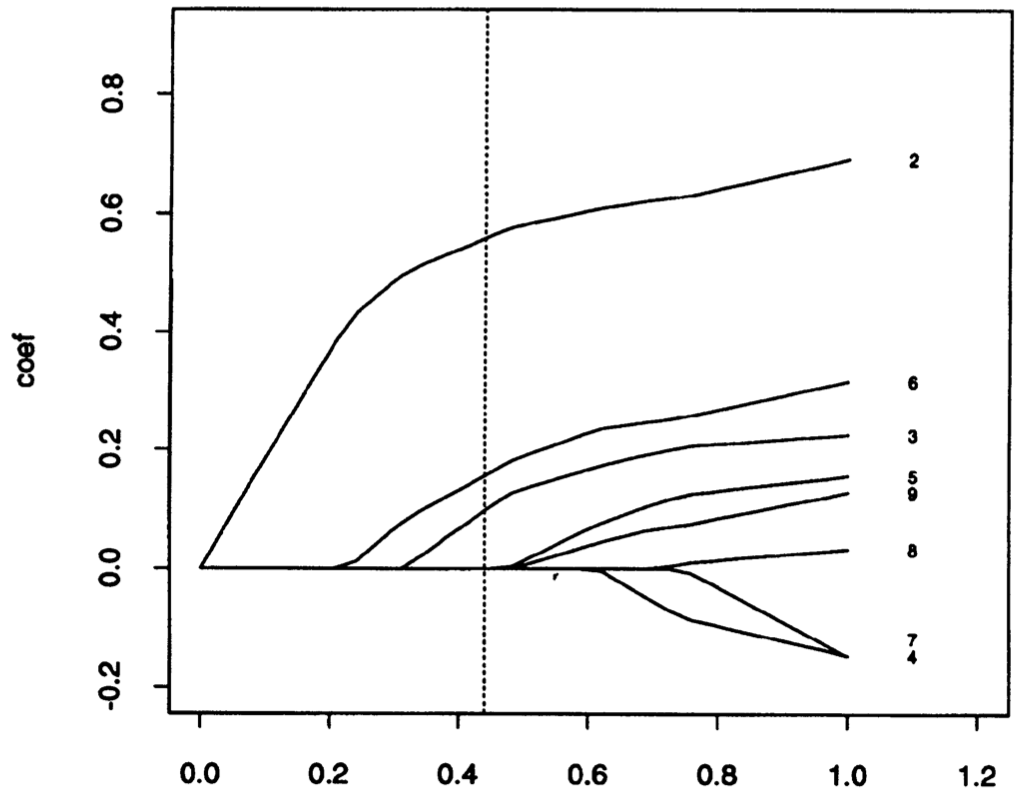
\includegraphics[scale=.25]{tibfig5}}
\center{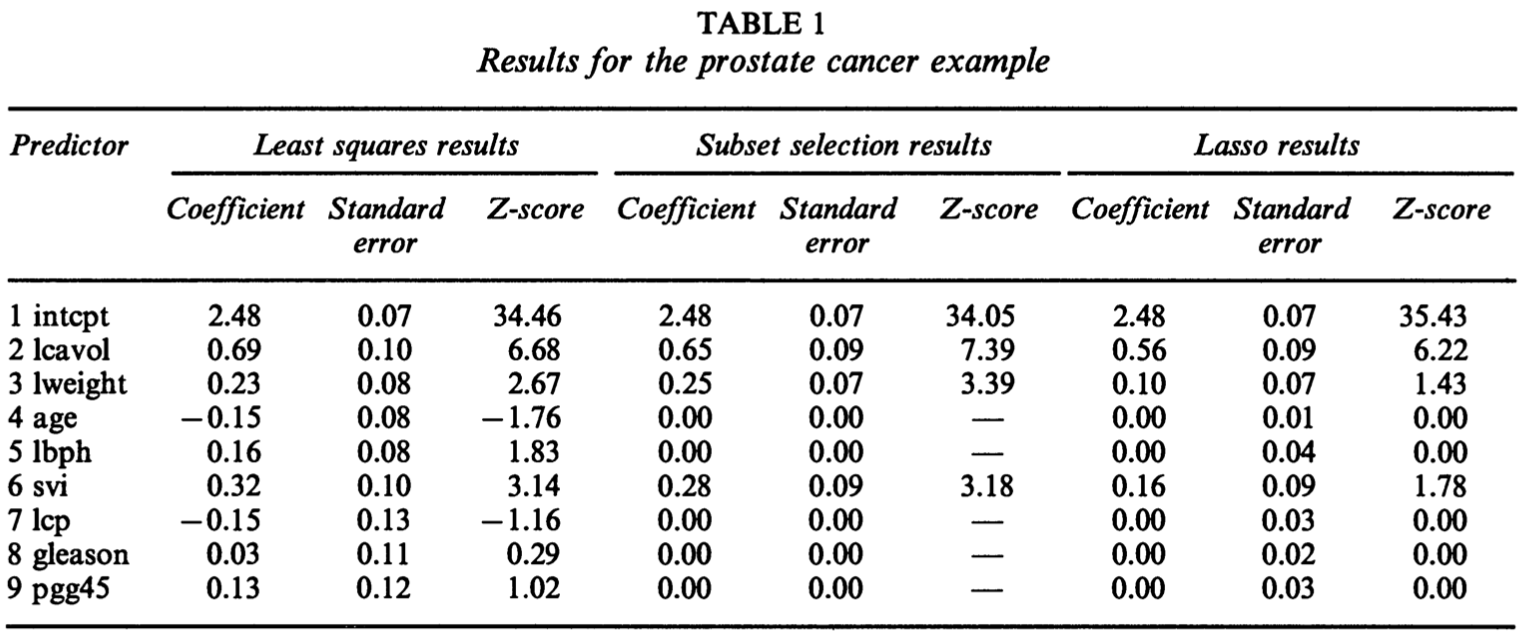
\includegraphics[scale=.25]{tibtable1}}

}



\subsection{Oil and Gas}
\subsection{House Prices}







%Simulations
\section{Simulation Analysis}

\frame{
\begin{multicols}{2}
 \tableofcontents[currentsection, hideothersubsections]
\end{multicols}
}

\frame{
\frametitle{Simulations}
\begin{itemize}
    \item 
    Tibshirani investigates several simulations testing Lasso alongside OLS, Ridge and subset selection
    \item
    This helps to shed some light on where lasso is most useful in the spectrum of options
    \item
    In these simulations we draw from a model of the form 
    \[
    y = \hat{\beta}^TX + \sigma \epsilon
    \]
    
\end{itemize}
}

\frame{
\frametitle{Simulation 1}
\begin{itemize}
    \item
    We have
$$
\beta = (3,1.5,0,0,2,0,0,0)^T
$$

    \item
    $\epsilon$ is standard normal, $\sigma = 3$ and the correlation between $x_i$ and $x_j$ is $\rho^{|i-j|}$ with $\rho = 0.5$
    
    \item
    50 samples were drawn at 20 observations each
    
    \item
    Both subset selection and Lasso will set some of the $\beta$'s to zero, we can compare how often models are produced with correct non-zero coefficients

\end{itemize}
}

\frame{
\begin{multicols}{2}

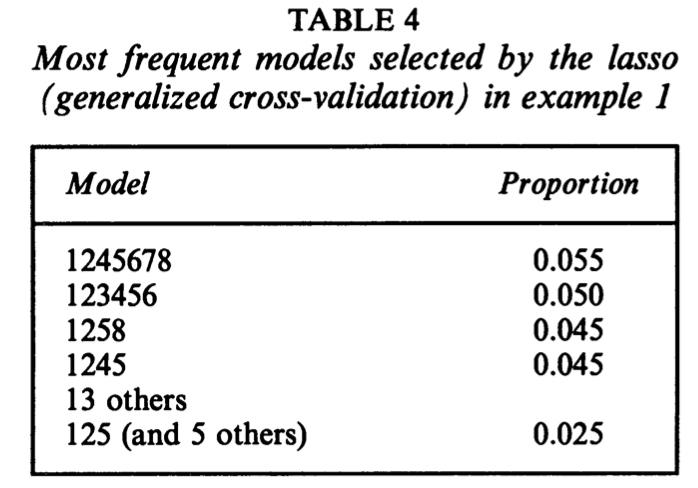
\includegraphics[scale=.45]{tibtable4}

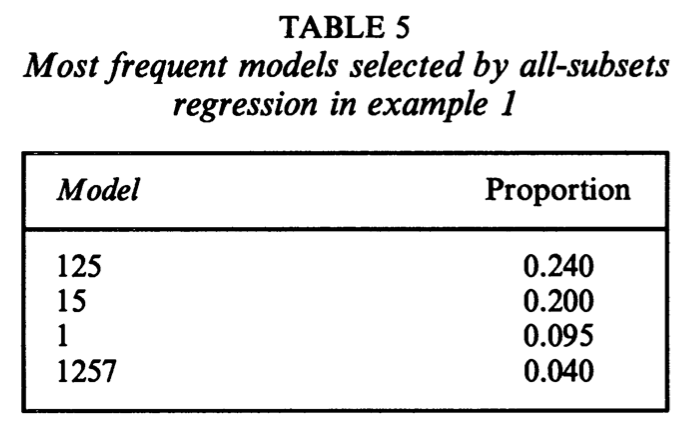
\includegraphics[scale=.45]{tibtable5}
\end{multicols}
Notice that although Lasso only chooses (1,2,5) 2.5\% of the time (1,2,5) are retained in 95.5\% of the models, where Subset has a tendency to under-fit.

}

\frame{
\frametitle{Simulation 1}

\center{Box and whisker plots of the coefficients are compared}

\begin{multicols}{2}
    ${}^1$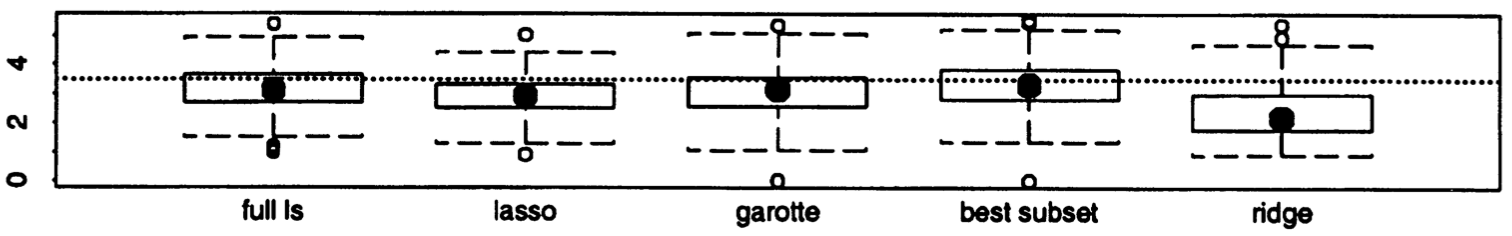
\includegraphics[scale = .22]{tibfig8-1}\\
    ${}^2$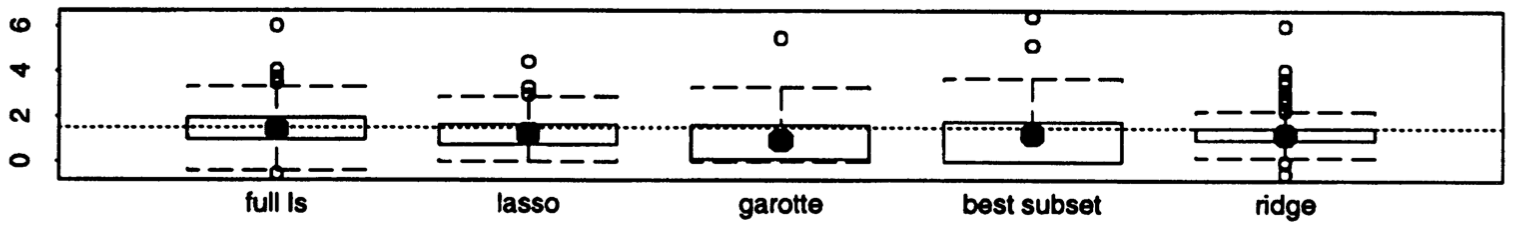
\includegraphics[scale = .22]{tibfig8-2}\\
    ${}^3$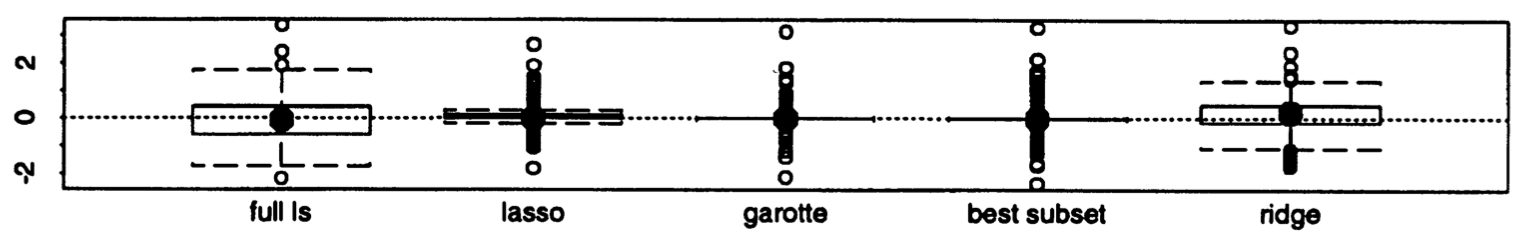
\includegraphics[scale = .22]{tibfig8-3}\\
    ${}^4$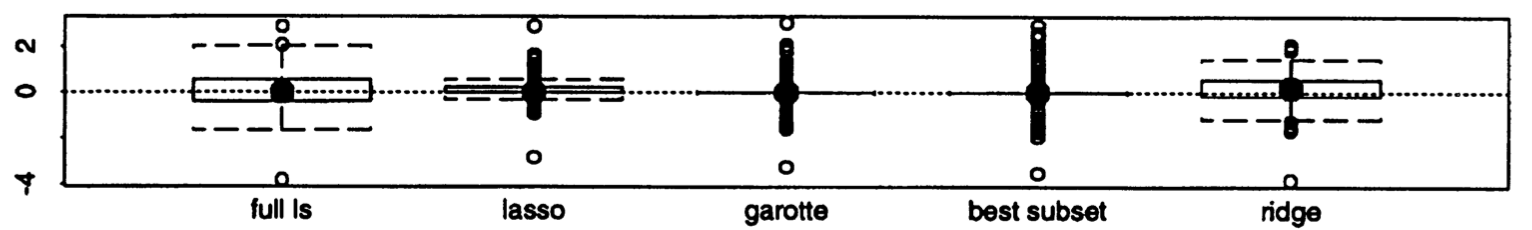
\includegraphics[scale = .22]{tibfig8-4}\\
    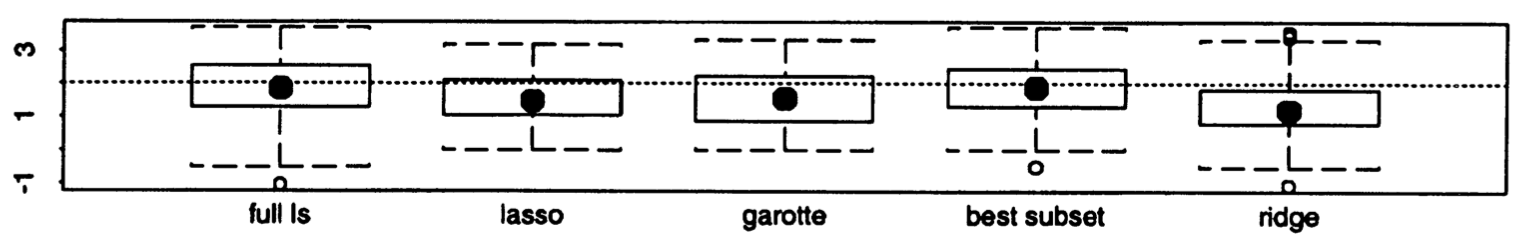
\includegraphics[scale = .22]{tibfig8-5}${}^5$\\
    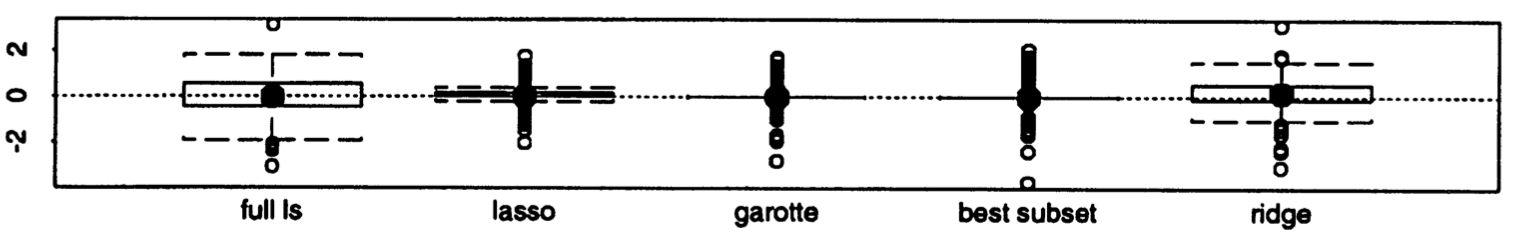
\includegraphics[scale = .22]{tibfig8-6}${}^6$\\
    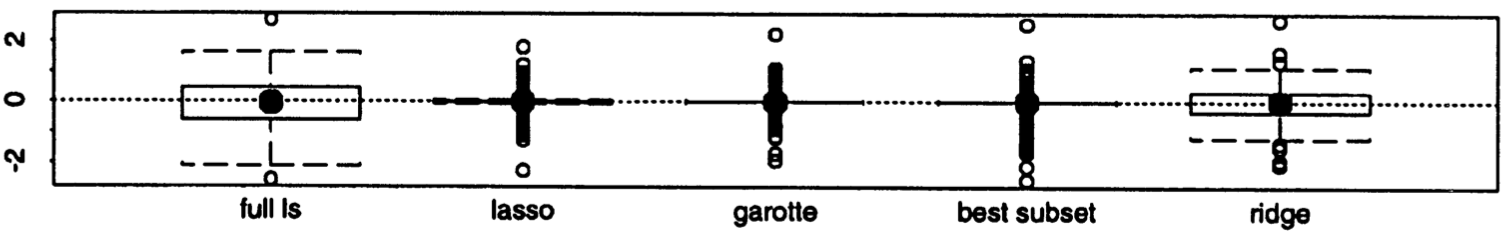
\includegraphics[scale = .22]{tibfig8-7}${}^7$\\
    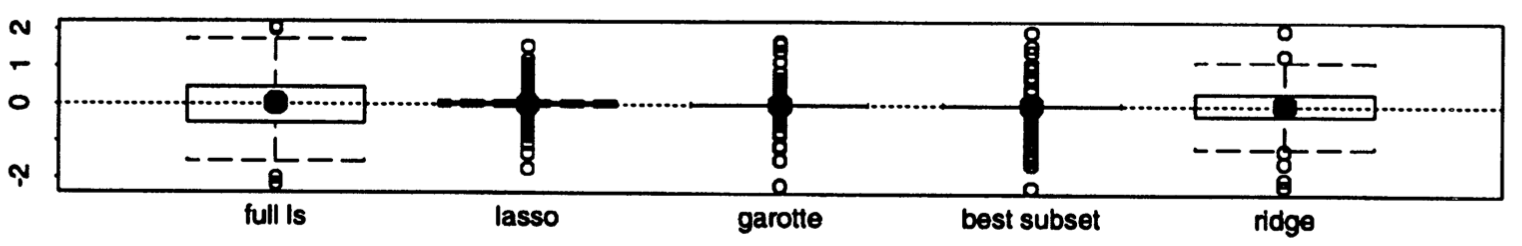
\includegraphics[scale = .22]{tibfig8-8}${}^8$\\
    
\end{multicols}    
Notice the variability on the OLS, Ridge and subset coefficients compared to Lasso

}

\frame{
\frametitle{Simulation2}
\begin{itemize}
\item
This is the same as simulation 1 but with $\beta = (0.85,0.85,0.85,0.85,0.85,0.85,0.85,0.85)^T$  and $\sigma = 3$

\item
In this data there is a large number of small effects
\end{itemize}
}

\frame{
\frametitle{Simulation2}
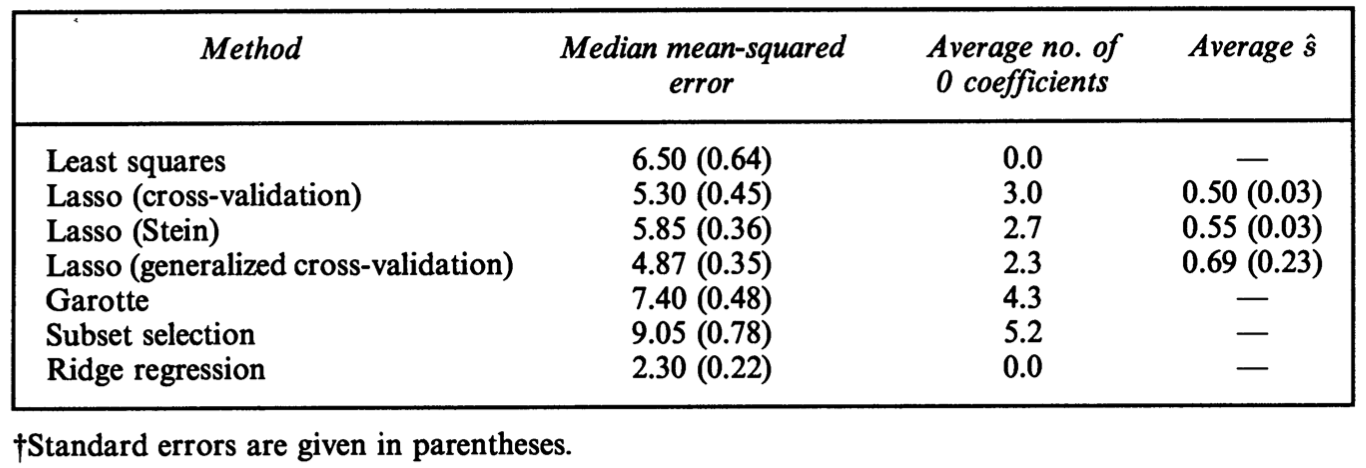
\includegraphics[scale = .4]{tibtable6}

}


\frame{
\frametitle{Simulation 3}
\center{$y = \hat{\beta}^TX + \sigma \epsilon$}\\

\begin{itemize}
\item 
In the 3rd simulation we let $\beta = (5,0,0,0,0,0,0,0)^T$ and $\sigma = 2$
\item 
This data should favor subset selection
\end{itemize}

}

\frame{
\frametitle{Simulation3}
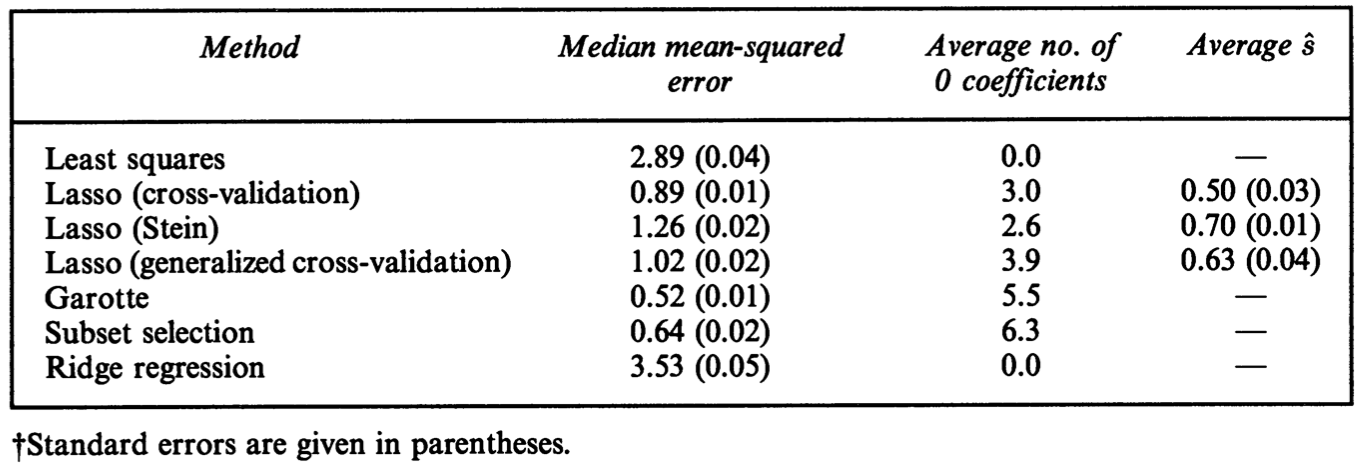
\includegraphics[scale = .4]{tibtable7}\\

We see that subset selection performs well as expected and Lasso is comparable 
}




%Adaptive Lasso
\section{Adaptive Lasso}

\frame{
\begin{multicols}{2}
 \tableofcontents[currentsection, hideothersubsections]
\end{multicols}
}

\frame{
    
    \begin{itemize}
        \item {\color{purple}$y_1= \beta_0 + \beta_1 x_1 + \beta_2 x_2+ \dots +\beta_{p-1} x_{p-1}$}
        \item
$
        \hat{\beta}(lasso) = \underset{\beta}{argmin} \norm{y- \sum_{j-1}^p x_j \beta_j}^2 + \lambda \sum_{j=1}^p |\beta|
$
\end{itemize}

}


\subsection{Oracle Property}
%Oracle Property










\section[Conclusion]{}

\frame{
    \frametitle{Lasso vs. Subset Selection vs. Ridge Regression}
    \begin{itemize}
        \item Small number of large effects.
        \begin{itemize}
            \item Subset selection is best, Lasso is second best, Ridge Regression is worst.
        \end{itemize}
        \item Small to moderate number of moderate-sized effects.
        \begin{itemize}
            \item Lasso is best, Ridge regression is second best, Subset selection is worst.
        \end{itemize}
        \item Large of small effects.
        \begin{itemize}
            \item Ridge regression is best, Lasso is second best, Subset selection is worst.
        \end{itemize}
    \end{itemize}
    
  
   
}


\frame{
    \frametitle{Lasso vs. Subset Selection vs. Ridge Regression}
    
    \begin{itemize}
        \item Do these results make sense?
        \begin{itemize}
            \item Recall that the Lasso was designed to work like Ridge regression but with some of the benefits of Subset selection.
            \item It thus makes sense for the Lasso to fall between Ridge regression and Subset selection on extreme cases and to beat both of them on cases not well-suited to either.
        \end{itemize}
        \item {\color{red} CAUTION!}
        \begin{itemize}
            \item These results refer to \color{red} prediction accuracy \color{black}
            \item As for {\color{blue} interpretability:}
            \begin{itemize}
                \item Subset selection $>$ Lasso $>$ Ridge regression, always
                \item Why? More nonzero coefficients = more interpretable, always
            \end{itemize}
        \end{itemize}
    \end{itemize}
}


\frame{
\frametitle{References}

}



\end{document}

